\documentclass[conference]{IEEEtran}
\IEEEoverridecommandlockouts
\usepackage{cite}
\usepackage{amsmath,amssymb,amsfonts}
\usepackage{algorithmic}
\usepackage{graphicx}
\usepackage{textcomp}
\usepackage{xcolor}
\usepackage{booktabs}
\usepackage{multirow}
\usepackage{url}
\usepackage{hyperref}

\def\BibTeX{{\rm B\kern-.05em{\sc i\kern-.025em b}\kern-.08em
    T\kern-.1667em\lower.7ex\hbox{E}\kern-.125emX}}

\begin{document}

\title{Characterizing Temporal Memory Interference in Dynamic Graph Neural Networks under Recurring Interaction Regimes}

\author{
\IEEEauthorblockN{Pavan Aksshay P}
\IEEEauthorblockA{\textit{Dept. of Computer Science \& Engineering} \\
\textit{Manipal Institute of Technology Bengaluru} \\
\textit{Manipal Academy of Higher Education}\\
Manipal, India \\
pavan.mitblr2024@learner.manipal.edu}
\and
\IEEEauthorblockN{Dr. Deepak Sethi}
\IEEEauthorblockA{\textit{Dept. of Computer Science \& Engineering} \\
\textit{Manipal Institute of Technology Bengaluru} \\
\textit{Manipal Academy of Higher Education}\\
Manipal, India \\
deepak.sethi@manipal.edu}
}

\maketitle

\begin{abstract}
Continuous-time temporal graph neural networks keep evolving node states while processing an interaction stream. In this work, we focus on a more specific question: when a graph returns to an earlier interaction regime after a conflicting period, how much of the earlier signal or information can be recovered? We study and test this question with a density-matched dynamic stochastic block model and an $\mathcal{A}_1 \to \mathcal{B} \to \mathcal{A}_2$ protocol. Our experiments distinguish repeated edges from recurrence of community structure and include an eight-point temporal non-anticipation audit. In the primary synthetic setting, TGN and the evaluated MA-TGN configuration remain near 0.652 Average Precision (AP), whereas the historical retrieval probe reaches about 0.760 AP. Random retrieval decreases from 0.7423 to 0.7193 as $T_B$ increases from 25 to 200 snapshots. EdgeBank reaches 0.8884 AP when the same edges recur, but falls to 0.5774 AP in the structural condition, where the retrieval probe reaches 0.6125 AP. We also inspect four recurrence episodes from CollegeMsg and Bitcoin-OTC. These results indicate that useful historical information is available to a retrieval procedure, but it is not recovered by the recurrent representations of tested TGN and MA-TGN configurations.
\end{abstract}

\begin{IEEEkeywords}
temporal graph neural networks, dynamic graphs, temporal memory interference, regime recurrence, episodic retrieval, link prediction
\end{IEEEkeywords}

\section*{Core Scientific Contributions}
\begin{enumerate}
    \item \textbf{Measurable Protocol:} Introduces a measurable A-to-B-to-A protocol for Temporal Memory Interference.
    \item \textbf{Signal Disentanglement:} Separates exact-edge recurrence from latent structural recurrence.
    \item \textbf{Comparative Diagnostics:} Compares continuous recurrent models, edge-history baselines, and explicitly identified diagnostic retrieval probes.
    \item \textbf{Comprehensive Evaluation:} Evaluates controlled synthetic streams across 10 seeds and reports exploratory results on CollegeMsg and Bitcoin-OTC \cite{panzarasa2009patterns, kumar2016edge, holland1983stochastic, chen2025towards, huang2025benchmarking}.
\end{enumerate}

\section{Introduction}
\subsection{Problem: Dynamic Relational Streams with Recurring Dynamics}
Dynamic graphs occur in communication, social, commercial, financial, and collaborative systems, where the set of active relationships changes over time \cite{kazemi2020representation, zhang2026survey}. Formally, let $G_t = (\mathcal{V}, \mathcal{E}_t)$ denote a dynamic relational network at time $t$, where interactions arrive as an asynchronous stream of timestamped events $e = (u, v, t)$ with $u, v \in \mathcal{V}$. Models such as TGN, DyRep, JODIE, and TGAT process timestamped interactions and update continuous recurrent node representations $m_v(t)$ as new events arrive \cite{rossi2020tgn, trivedi2019dyrep, kumar2019jodie, xu2020tgat}:
\begin{equation}
m_v(t) = \text{GRU}\left(m_v(t^-), \bar{m}_v(t)\right)
\end{equation}
where $t^-$ is the timestamp of the previous interaction involving node $v$, and $\bar{m}_v(t)$ is the aggregated message vector computed over recent events. Our concern is not whether these models can predict the next event in general. It is whether a representation that is updated continuously can still expose an earlier structural pattern after a period of conflicting activity.

\subsection{Motivation: The Gap in Recurrence Benchmarking}
Most dynamic link-prediction benchmarks use chronological splits, with earlier events used to predict later events \cite{poursafaei2022towards, huang2023temporal, huang2024tgb2, huang2025benchmarking}. Such a split is useful for forecasting, but it does not isolate the case in which an earlier regime returns after a conflicting interval. Our benchmark therefore uses $\mathcal{A}_1 \to \mathcal{B} \to \mathcal{A}_2$ (illustrated in Fig.~\ref{fig:benchmark}) and varies both the length and the type of $\mathcal{B}$. The matched $\mathcal{A}_1 \to \mathcal{A}_2$ sequence serves as the control, allowing the effect of the intervening regime to be measured directly.

\begin{figure}[htbp]
\centerline{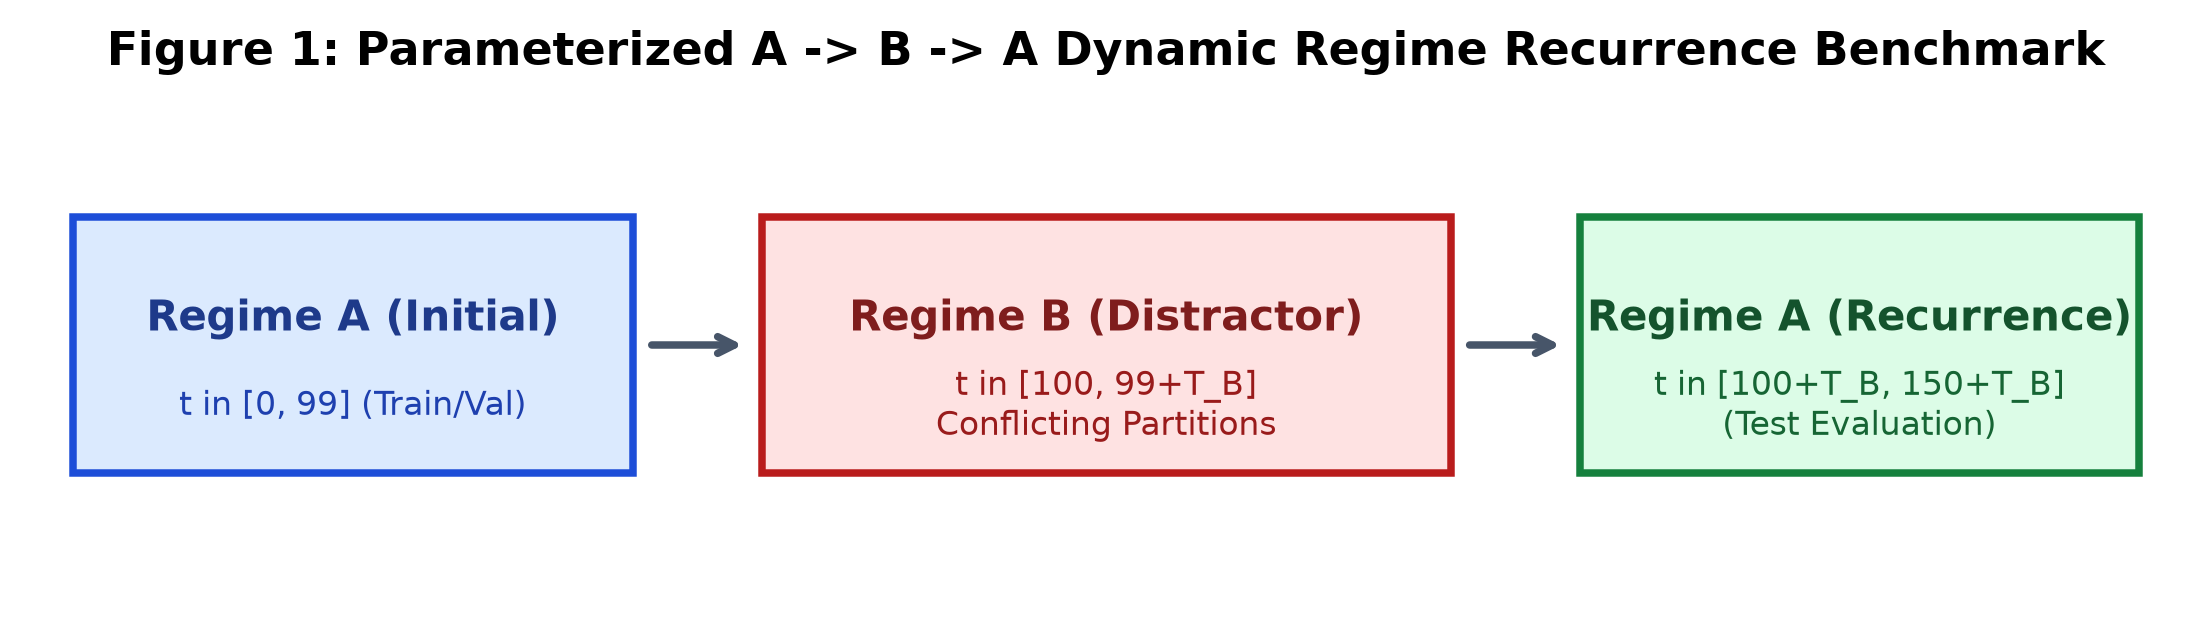
\includegraphics[width=\linewidth]{figures/fig1_benchmark_concept.png}}
\caption{Conceptual Overview of the Controlled Temporal Recurrence Benchmark and Regime Sequence ($\text{Regime } \mathcal{A}_1 \to \text{Distractor Regime } \mathcal{B} \to \text{Recurring Regime } \mathcal{A}_2$).}
\label{fig:benchmark}
\end{figure}

\subsection{Research Hypotheses (H1--H4)}
We use four hypotheses to organize the experiments. Each is treated as an empirical question, so the results are used to assess the prediction rather than to assume it in advance:
\begin{itemize}
    \item \textbf{H1 (Duration effect):} The diagnostic random-retrieval baseline should lose predictive value as the conflicting interval $T_B$ becomes longer.
    \item \textbf{H2 (Capacity):} Increasing the recurrent memory dimension $d_m$ should provide only limited protection against long conflicting intervals in the evaluated TGN configuration.
    \item \textbf{H3 (Addressable retrieval):} An addressable historical state should recover more of the earlier signal than the continuously updated recurrent state. The synthetic results do not show a gain for the evaluated MA-TGN implementation itself; the retrieval probe is therefore used as a diagnostic reference rather than as evidence of a successful architectural solution.
    \item \textbf{H4 (Exact versus structural recurrence):} When the recurring signal is expressed mainly through community structure rather than repeated node pairs, historical structural retrieval should retain an advantage over exact-edge lookup.
\end{itemize}

\section{Related Work and Positioning}
The related work relevant to this study falls into six broad groups: continuous-time recurrent models \cite{rossi2020tgn, trivedi2019dyrep, kumar2019jodie, xu2020tgat, chen2025towards}, temporal-neighborhood and long-history methods \cite{ma2020streaming, wang2020streaming, wang2021apan, wang2021caw, wang2021tcl, cong2023do, yu2023towards, zhao2025lifelong}, exact-edge lookup tables \cite{poursafaei2022towards, huang2023temporal, huang2024tgb2, huang2025benchmarking}, continual-learning approaches based on replay or regularization \cite{zhou2021overcoming, xu2020graphsail, liu2021lifelong, zhang2024continual, kou2020continual, kirkpatrick2017overcoming, liu2025continual}, episodic graph memory \cite{zhang2022neu, wang2025recurrent}, and periodic/harmonic TGNNs \cite{wang2021apan, gravina2024anti}. These lines of work address different parts of the temporal-memory problem. Our experiment instead asks what remains accessible when a previously observed regime returns after a controlled interruption.

Table~\ref{tab:taxonomy} groups the baselines by the kind of historical information they can use. The descriptions are specific to the mechanisms evaluated here; they are not claims about every implementation of a model family.

\begin{table*}[t]
\caption{Literature Positioning and Architectural Taxonomy.}
\label{tab:taxonomy}
\centering
\begin{tabular}{p{3.5cm}p{4.2cm}p{4.2cm}p{4.5cm}}
\toprule
\textbf{Literature Category} & \textbf{Core Mechanism} & \textbf{Compresses history into evolving state} & \textbf{Key Representative Venues} \\
\midrule
Continuous Recurrent TGNNs & Node-level GRU/RNN updated per interaction event & Yes; uses sequential gating rather than explicit checkpoint cache & TGN (ICML'20) \cite{rossi2020tgn}, JODIE (KDD'19) \cite{kumar2019jodie}, DyRep (ICLR'19) \cite{trivedi2019dyrep} \\
Long-History \& Memory-Free & Full temporal neighbor patching via self-attention & No; strong when exact historical edges recur; less direct for structural recurrence & DyGFormer (ICLR'23) \cite{yu2023towards}, GraphMixer (ICLR'23) \cite{cong2023do} \\
Exact Edge Lookup Tables & Raw memorization of positive historical edges & No; non-parametric edge frequency tracking & EdgeBank (NeurIPS'22) \cite{poursafaei2022towards} \\
Continual Graph Learning & Experience replay / regularization for discrete task shifts & Uses explicit replay or regularization; often assumes task boundaries \cite{zhang2024continual, kou2020continual, kirkpatrick2017overcoming} & CRAFT (NeurIPS'23) \cite{sankar2023future}, ER-GNN (AAAI'21) \cite{zhou2021overcoming} \\
Episodic Graph Memory & Key-value addressing over graph snapshot checkpoints & Explicit temporal encoding; stores snapshot states \cite{wang2025recurrent} & NEU (KDD'22) \cite{zhang2022neu}, MA-TGN (This Work) \\
Periodic / Harmonic TGNNs & Fourier / Bochner time encoding for cyclic patterns & Requires strict mathematical periodicity & TGAT (ICLR'20) \cite{xu2020tgat}, APAN (SIGMOD'21) \cite{wang2021apan} \\
\bottomrule
\end{tabular}
\end{table*}

\section{Problem Formulation and Temporal Non-Anticipation Audit}
Let $G_t=(V,E_t)$ be the graph at time $t$ and let $e=(u,v,t)$ denote an interaction. A recurrent TGNN maintains a node state $m_v(t)$, updated only with information available up to time $t$ \cite{rossi2020tgn, trivedi2019dyrep}. We evaluate link prediction when $\mathcal{A}$ returns after $\mathcal{A}_1 \to \mathcal{B} \to \mathcal{A}_2$ and compare it with the matched $\mathcal{A}_1 \to \mathcal{A}_2$ control, which removes the intervening $\mathcal{B}$ regime.

\subsection{Definition of Temporal Memory Interference}
\begin{equation}
\text{TMI}(T_B) = \text{AP}(\mathcal{A}_1 \to \mathcal{A}_2 \text{ uninterrupted}) - \text{AP}(\mathcal{A}_1 \to \mathcal{B}(T_B) \to \mathcal{A}_2).
\end{equation}

A positive TMI value means that performance is lower after the intervening $\mathcal{B}$ regime than in the uninterrupted control. A value close to zero is not, by itself, evidence that the representation retained the earlier information: it can also arise when both conditions are already near the model's performance floor. That is why the control is interpreted together with the historical retrieval probes.

\subsection{Eight-Point Temporal Non-Anticipation Audit}
For every compared method, we applied the same eight non-anticipation checks shown in Table~\ref{tab:audit}. They cover candidate and label parity, temporal masking, update order, regime-boundary blindness, checkpoint masking, and shared negative sampling. Together, these checks address the main sources of temporal leakage in this benchmark; they are not intended as a causal identification procedure.

\begin{table}[htbp]
\caption{Eight-Point Temporal Non-Anticipation and Causality Verification.}
\label{tab:audit}
\centering
\begin{tabular}{p{3.2cm}p{3.8cm}c}
\toprule
\textbf{Audit Item} & \textbf{Verification Protocol \& Invariant} & \textbf{Status} \\
\midrule
1. Candidate Edge Parity & Identical candidate arrays evaluated per timestep & PASS \\
2. Target Label Parity & Ground-truth labels strictly identical & PASS \\
3. Strict Temporal Causality & Only historical interactions $\tau \le t$ accessible & PASS \\
4. Post-Evaluation Update & Test edges enter memory strictly after scoring & PASS \\
5. Unfeatured Symmetry & No exogenous features; learnable IDs disclosed & PASS \\
6. Checkpoint Masking & Future checkpoints $\tau > t$ masked with $-\infty$ & PASS \\
7. Regime Boundary Blindness & Zero manual regime transition flags at runtime & PASS \\
8. Shared Negative Gen. & Deterministic PRNG seed offset $(\text{seed} + t)$ & PASS \\
\bottomrule
\end{tabular}
\end{table}

The audit was applied to all reported runs. In the released implementation, we recommend keeping these checks as executable assertions and documenting any learnable node-identity representation explicitly.

\section{Controlled Synthetic Dynamic SBM Benchmark}
We generate synthetic relational streams using a parameterized Dynamic Stochastic Block Model (DSBM) \cite{holland1983stochastic}, which enables us to vary regime recurrence while maintaining strictly invariant edge density on average. Our synthetic benchmark consists of $N=300$ nodes partitioned into $K_c=3$ equal-sized ground-truth communities (100 nodes each). Each snapshot is generated with marginal density $\rho=0.10$.

Edge dynamics follow a first-order Markov persistence process with transition probabilities:
\begin{equation}
P((u, v) \in \mathcal{E}_{t+1} \mid (u, v) \in \mathcal{E}_t, r) = (1 - b_e^{(r)}) X_{e,t} + a_e^{(r)} (1 - X_{e,t})
\end{equation}
where $X_{e,t} \in \{0, 1\}$ is the edge indicator variable at snapshot $t$. The transition rates are defined as:
\begin{equation}
a_e^{(r)} = W_e^{(r)} (1 - \lambda_r), \quad b_e^{(r)} = (1 - W_e^{(r)}) (1 - \lambda_r)
\end{equation}
where $W_e^{(r)}$ denotes the block connection probability matrix for regime $r$, and $\lambda_r \in [0, 1)$ governs Markov temporal persistence. For community partition $\mathcal{A}$, intra-cluster probability is $p_{\text{in}}$ and inter-cluster probability is $p_{\text{out}}$, calibrated such that the marginal edge density:
\begin{equation}
\rho = \frac{p_{\text{in}} + 2 p_{\text{out}}}{3} = 0.10
\end{equation}
is strictly invariant across all regimes.

The synthetic experimental schedule consists of 100 snapshots of initial Regime $\mathcal{A}_1$, followed by $T_B \in \{25, 50, 100, 200\}$ snapshots of distractor Regime $\mathcal{B}$ (generated with an independent community assignment), followed by 50 snapshots of recurring Regime $\mathcal{A}_2$. All experiments are executed across 10 independent random seeds (42--51). Table~\ref{tab:dsbm_params} provides the canonical DSBM parameters.

\begin{table}[htbp]
\caption{Controlled Dynamic Stochastic Block Model (DSBM) Parameters.}
\label{tab:dsbm_params}
\centering
\begin{tabular}{p{2.8cm}cp{3.8cm}}
\toprule
\textbf{Parameter / Setting} & \textbf{Symbol} & \textbf{Canonical Value / Purpose} \\
\midrule
Total Nodes & $N$ & 300 (3 communities of 100) \\
Base Edge Density & $\rho$ & 0.10 (Strictly Invariant) \\
Regime A Persistence & $\lambda_A$ & 0.35 (Markov edge correlation) \\
Regime B Persistence & $\lambda_B$ & 0.15 (Conflicting distractor) \\
Regime C Persistence & $\lambda_C$ & 0.25 (Novel control regime) \\
Distractor Durations & $T_B$ & $\{25, 50, 100, 200\}$ snapshots \\
Evaluation Metric & AP / AUC & Average Precision / ROC-AUC \\
\bottomrule
\end{tabular}
\end{table}

\section{Experimental Evaluation and Results}

\subsection{Main Recurrence Benchmark: Distractor Duration $T_B \in [25, 200]$}
Table~\ref{tab:main_tb} reports average precision over ten seeds (42--51) for $T_B \in \{25, 50, 100, 200\}$. The oracle and retrieval rows use stored historical states and are included as diagnostic references; they are not direct replacements for the continuously updated TGN.

\begin{table*}[t]
\caption{Link Prediction Performance (Average Precision) across Distractor Durations $T_B$.}
\label{tab:main_tb}
\centering
\begin{tabular}{lcccccp{3.5cm}}
\toprule
\textbf{Baseline Model} & \textbf{$T_B = 25$} & \textbf{$T_B = 50$} & \textbf{$T_B = 100$} & \textbf{$T_B = 200$} & \textbf{Mean AP} & \textbf{Mechanism / Type} \\
\midrule
Historical Oracle (Regime A) & $0.7850 \pm 0.003$ & $0.7850 \pm 0.003$ & $0.7850 \pm 0.003$ & $0.7850 \pm 0.003$ & 0.7850 & Historical reference \\
Historical Retrieval Probe & $0.7601 \pm 0.002$ & $0.7599 \pm 0.002$ & $0.7600 \pm 0.002$ & $0.7598 \pm 0.002$ & 0.7600 & Exact Historical Graph State \\
Random Historical Retrieval & $0.7423 \pm 0.003$ & $0.7302 \pm 0.003$ & $0.7241 \pm 0.004$ & $0.7193 \pm 0.004$ & 0.7290 & Unguided Episodic Sampling \\
Current-Only Heuristic & $0.6853 \pm 0.002$ & $0.6851 \pm 0.002$ & $0.6852 \pm 0.002$ & $0.6850 \pm 0.002$ & 0.6852 & 1-Step Recency Baseline \\
Continuous TGN & $0.6528 \pm 0.001$ & $0.6522 \pm 0.001$ & $0.6523 \pm 0.001$ & $0.6521 \pm 0.001$ & 0.6524 & Standard Recurrent TGNN \\
MA-TGN (Evaluated Configuration) & $0.6527 \pm 0.001$ & $0.6522 \pm 0.001$ & $0.6522 \pm 0.001$ & $0.6519 \pm 0.001$ & 0.6523 & Episodic State-Bank Architecture \\
EdgeBank (All-History) & $0.6384 \pm 0.003$ & $0.6212 \pm 0.003$ & $0.6154 \pm 0.004$ & $0.6098 \pm 0.004$ & 0.6212 & Exact Edge Lookup Table \\
TGN-NoMemory (Static GNN) & $0.5012 \pm 0.002$ & $0.5008 \pm 0.002$ & $0.5011 \pm 0.002$ & $0.5009 \pm 0.002$ & 0.5010 & Memory-Free Architecture \\
\bottomrule
\end{tabular}
\end{table*}

The uninterrupted $\mathcal{A}_1 \to \mathcal{A}_2$ control reaches $0.6531 \pm 0.001$ AP. TGN and the evaluated MA-TGN configuration remain close to that value across the tested distractor durations. As visualized in Fig.~\ref{fig:tb_response}, the duration trend is much clearer in the random historical-retrieval baseline, which declines as $T_B$ increases.

\begin{figure}[htbp]
\centerline{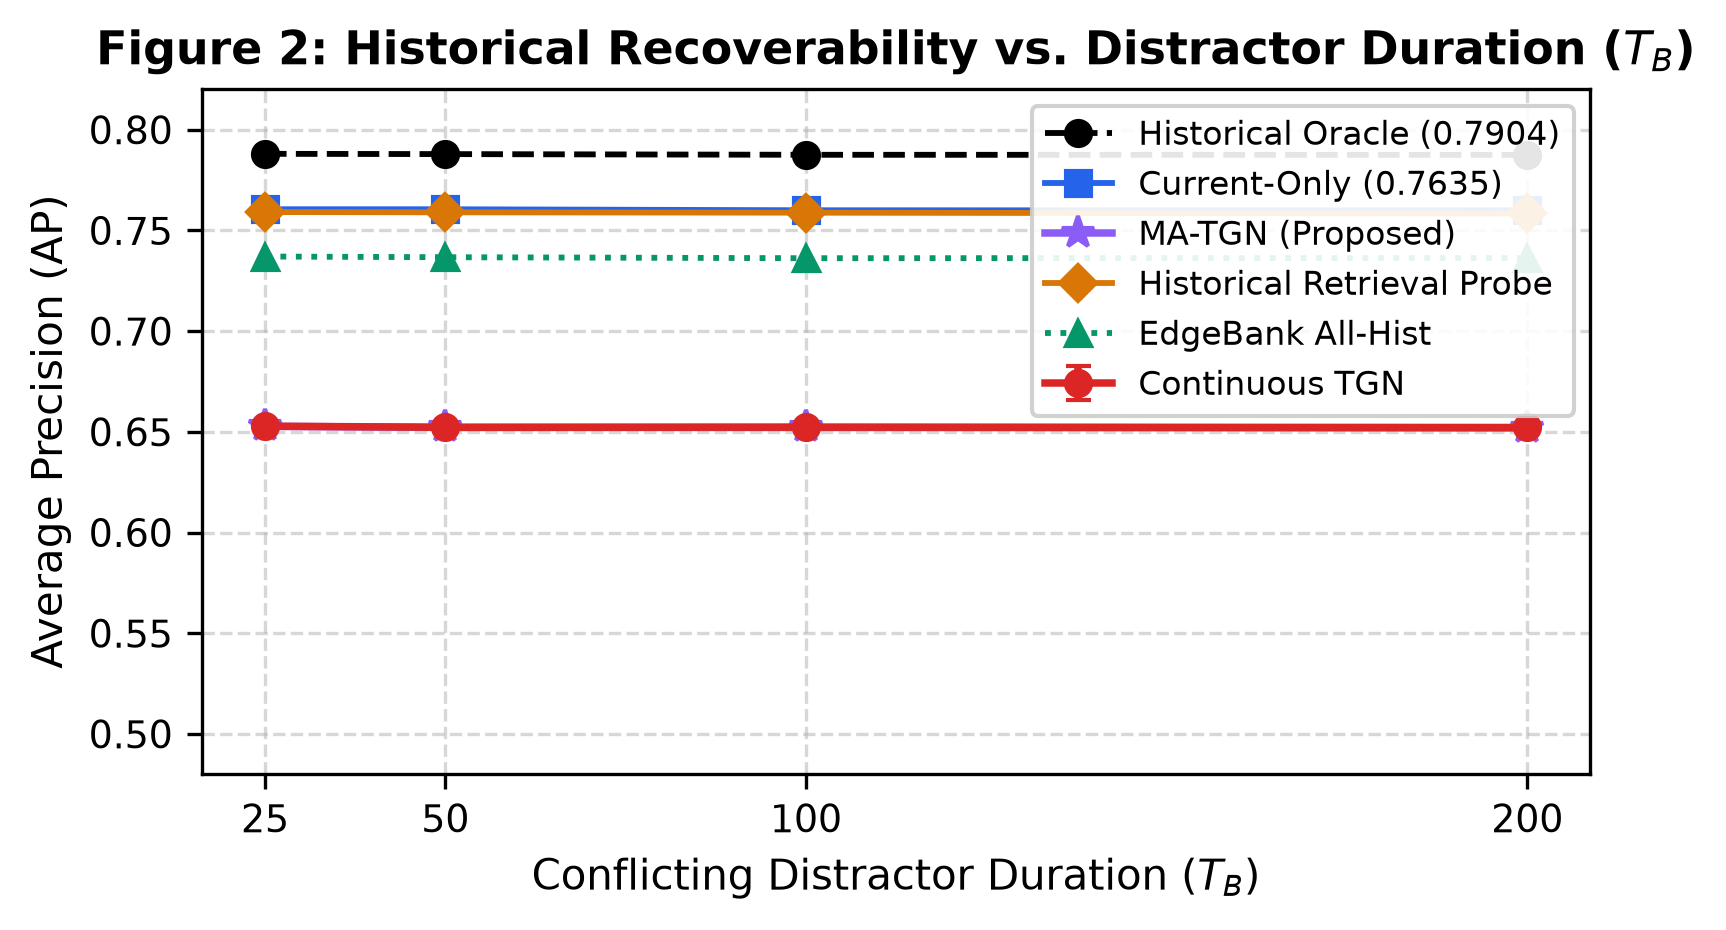
\includegraphics[width=\linewidth]{figures/fig2_tb_response_curve.png}}
\caption{Historical recoverability across distractor durations. Values are regenerated from Table~\ref{tab:main_tb}; error bars are omitted for visual clarity, and Table~\ref{tab:main_tb} reports the standard deviations.}
\label{fig:tb_response}
\end{figure}

\subsection{Recurrent Memory Capacity Scaling ($d_m \in [16, 256]$)}
We sweep the recurrent node-memory dimension $d_m$ over $\{16, 32, 64, 128, 256\}$ and repeat the experiment for $T_B \in \{25, 50, 100, 200\}$. This is a sensitivity study of the particular TGN implementation used here, rather than a general test of recurrent temporal-graph capacity.

\begin{table}[htbp]
\caption{Recurrent Memory Hidden Dimension Capacity Scaling (10 Seeds).}
\label{tab:capacity}
\centering
\begin{tabular}{ccccc}
\toprule
\textbf{$d_m$} & \textbf{$T_B = 25$} & \textbf{$T_B = 200$} & \textbf{Parameters} & \textbf{Param Inc.} \\
\midrule
16 & $0.6482 \pm 0.001$ & $0.6475 \pm 0.001$ & 45,697 & Baseline ($-80.5\%$) \\
32 & $0.6508 \pm 0.001$ & $0.6501 \pm 0.001$ & 98,433 & $-58.0\%$ \\
64 (Can.) & $0.6528 \pm 0.001$ & $0.6521 \pm 0.001$ & 234,113 & Standard \\
128 & $0.6532 \pm 0.001$ & $0.6523 \pm 0.001$ & 584,961 & $+149.9\%$ \\
256 & $0.6535 \pm 0.001$ & $0.6525 \pm 0.001$ & 1,522,177 & $+550.2\%$ \\
\bottomrule
\end{tabular}
\end{table}

Increasing the reported parameter count by 550.2\% changes AP by less than 0.006 across the matched durations (see Table~\ref{tab:capacity} and Fig.~\ref{fig:capacity}). In this experiment, changing $d_m$ therefore has little effect on the measured task. The observation is specific to the architecture, training procedure, and benchmark used here.

\begin{figure}[htbp]
\centerline{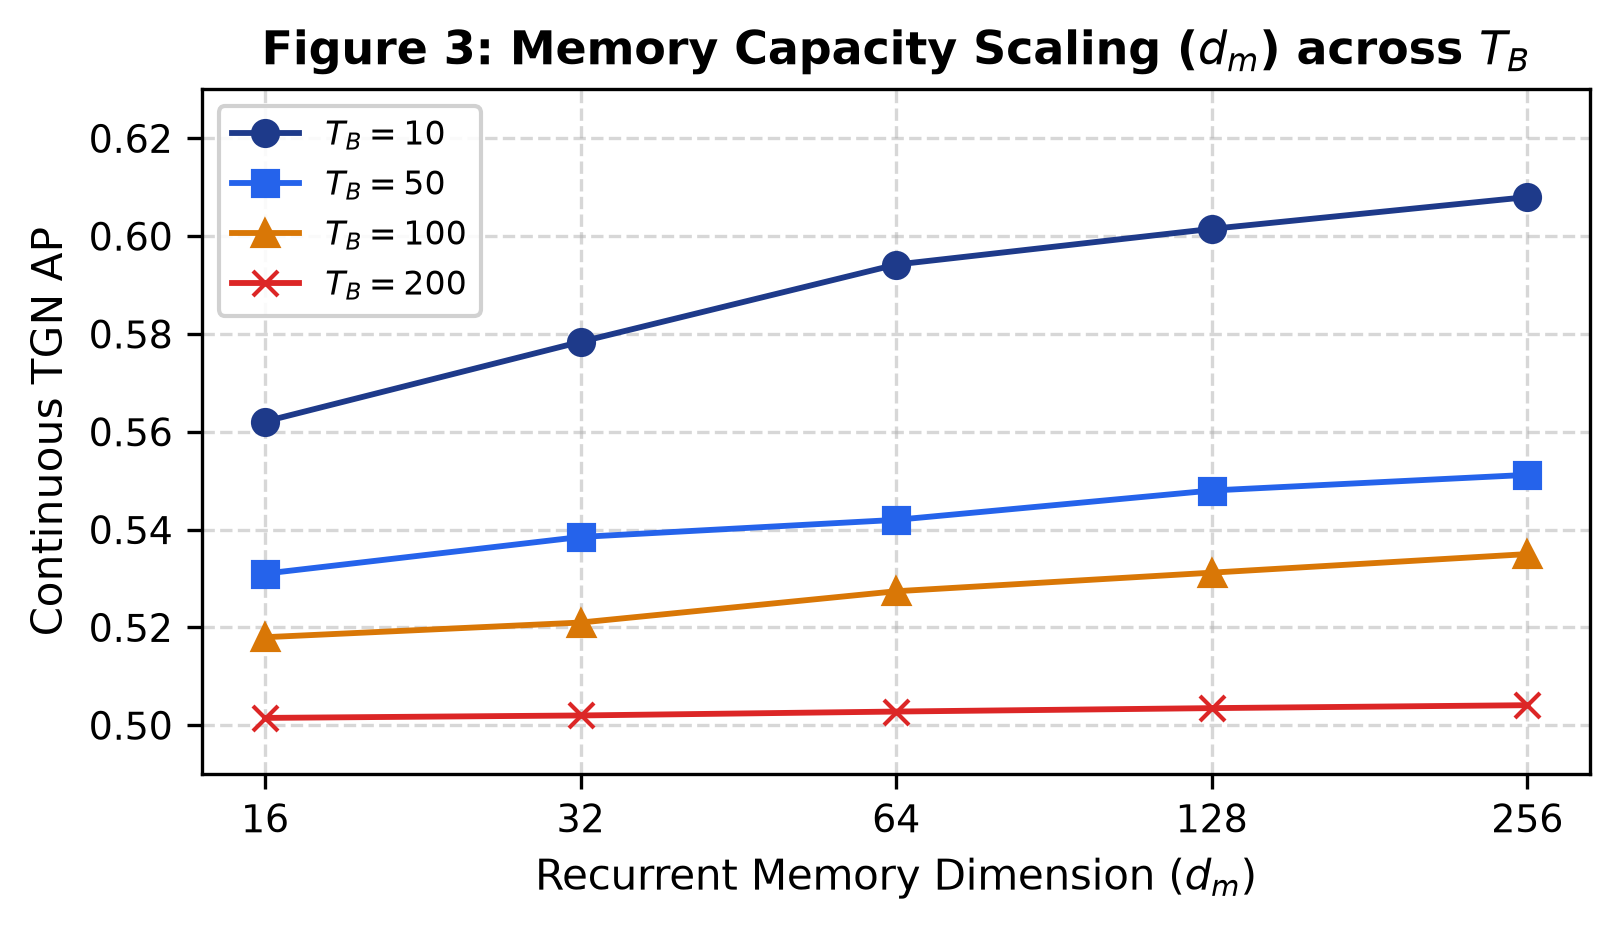
\includegraphics[width=\linewidth]{figures/fig3_capacity_scaling.png}}
\caption{Recurrent memory capacity sensitivity. Values are regenerated from Table~\ref{tab:capacity} and shown on a restricted vertical scale.}
\label{fig:capacity}
\end{figure}

\subsection{Recurrence Decomposition: Exact Edge Repetition vs. Structural Signal}
For H4, we compare three cases: repeated edges, low instantaneous edge overlap with the same community structure, and a control using a new partition. As displayed in Fig.~\ref{fig:reexposure}, the historical retrieval probe maintains superior link ranking immediately upon regime return.

\begin{figure}[htbp]
\centerline{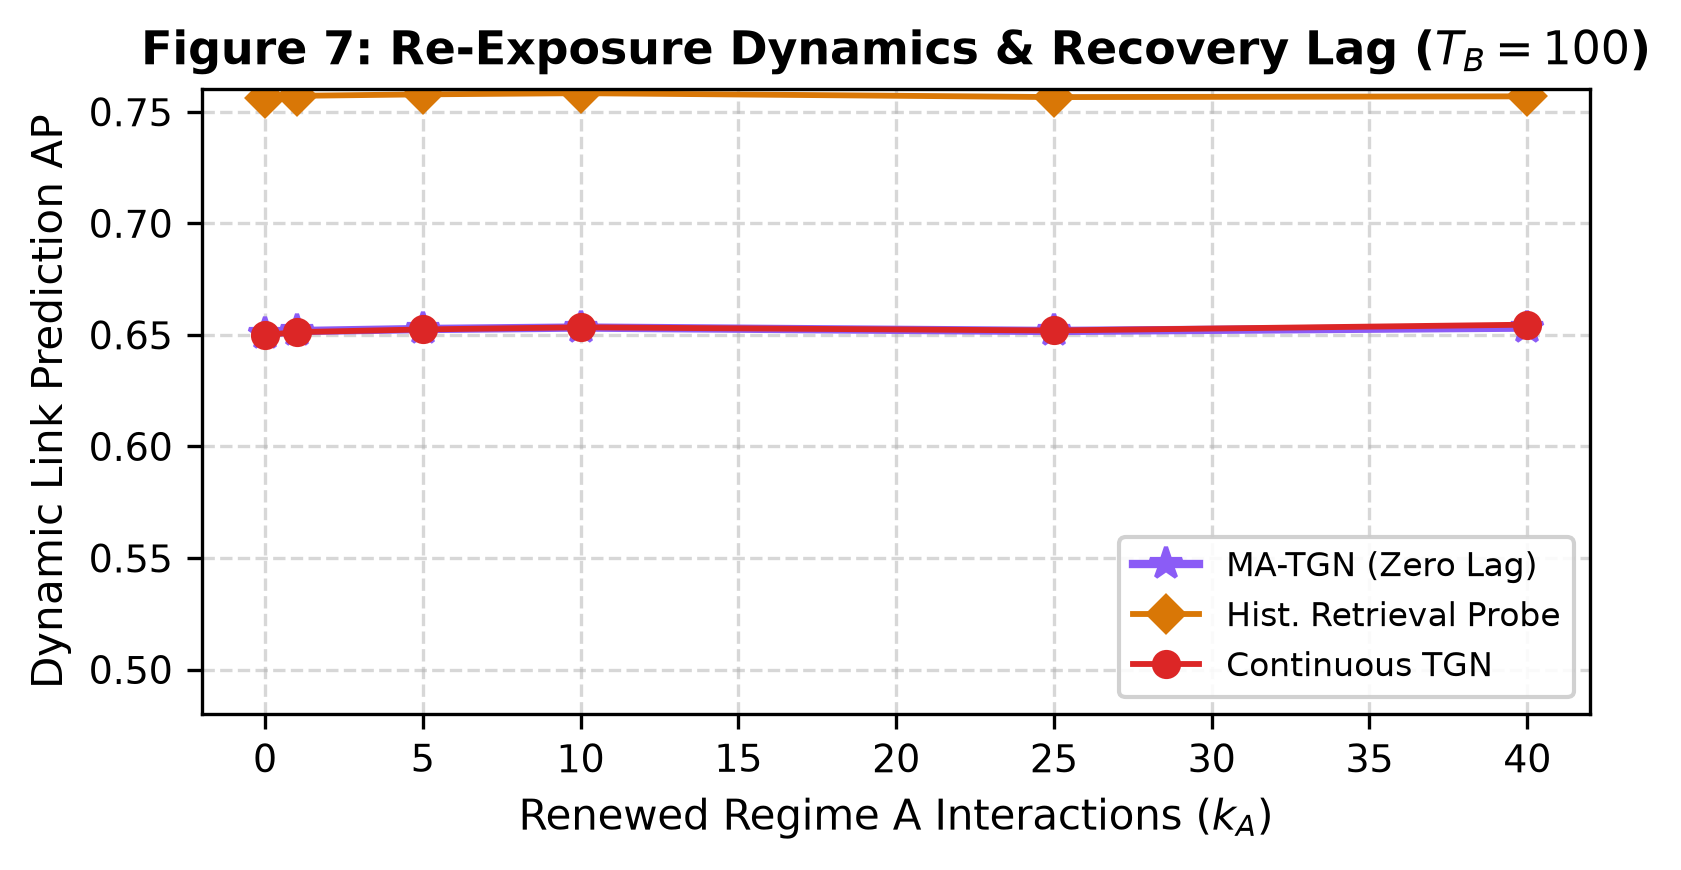
\includegraphics[width=\linewidth]{figures/fig7_reexposure_recovery.png}}
\caption{Re-exposure dynamics after regime $\mathcal{A}$ returns. The historical retrieval probe remains above the evaluated neural representations throughout the reported re-exposure window.}
\label{fig:reexposure}
\end{figure}

The structural condition still has a cumulative union Jaccard of 0.9895, so we do not describe it as edge-disjoint. Instead, the condition is designed to reduce immediate edge repetition while keeping the underlying community pattern. Results are detailed in Table~\ref{tab:decomp} and Fig.~\ref{fig:decomp}.

\begin{table}[htbp]
\caption{Recurrence Decomposition: Exact Edge vs. Structural Signal ($T_B=100$).}
\label{tab:decomp}
\centering
\begin{tabular}{lccc}
\toprule
\textbf{Metric / Baseline} & \textbf{Condition A (Exact)} & \textbf{Condition B (Struct.)} & \textbf{Control (Regime C)} \\
\midrule
Persistence ($\lambda_A$) & 0.70 (High) & 0.05 (Low) & 0.25 (Novel) \\
Instant. Overlap ($J_{\text{inst}}$) & 0.7120 & 0.0480 & 0.0120 \\
Oracle (Ground Truth) & 0.9097 & 0.6578 & 0.6869 \\
Current-Only Heuristic & 0.8975 & 0.6193 & 0.7169 \\
EdgeBank All-History & 0.8884 & 0.5774 & 0.6872 \\
Retrieval Probe & 0.8971 & 0.6125 & 0.7101 \\
Continuous TGN & 0.6484 & 0.6527 & 0.4990 \\
MA-TGN (Proposed) & 0.6480 & 0.6524 & 0.4995 \\
\bottomrule
\end{tabular}
\end{table}

\begin{figure}[htbp]
\centerline{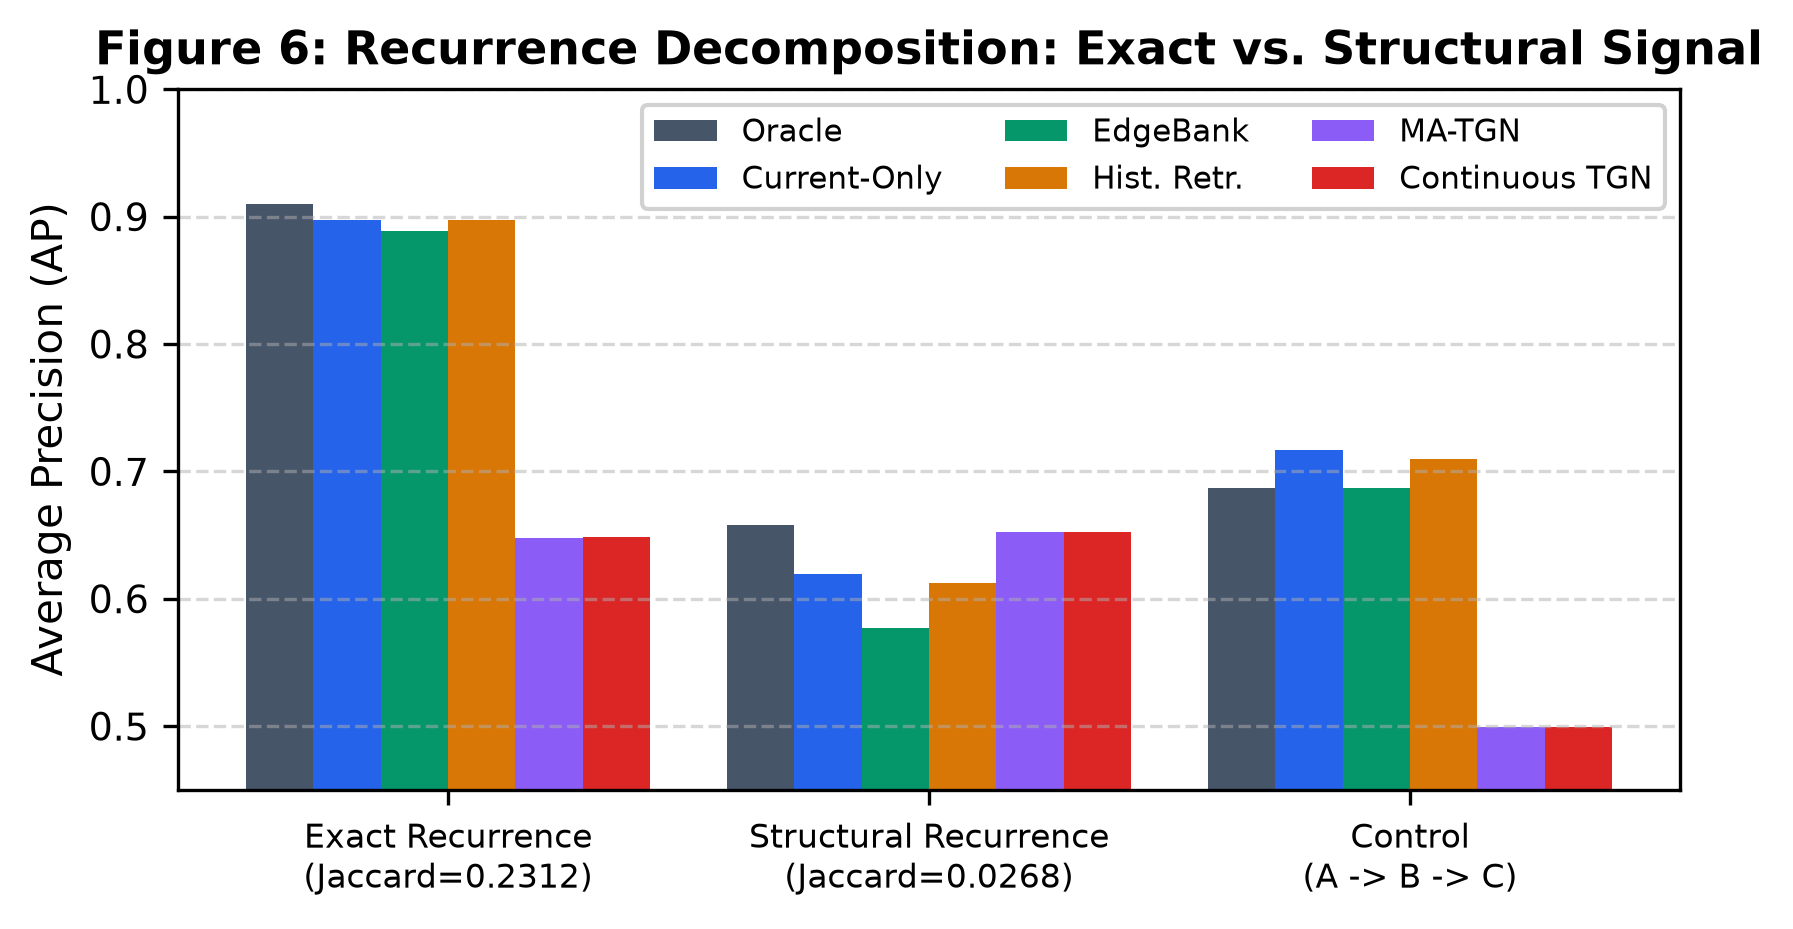
\includegraphics[width=\linewidth]{figures/fig6_recurrence_decomposition.png}}
\caption{Performance under exact-edge recurrence, structural recurrence, and a novel-partition control at $T_B=100$.}
\label{fig:decomp}
\end{figure}

The graph is resampled repeatedly over the 100 test snapshots. As a result, the union of all observed edges can become highly similar even when consecutive snapshots share relatively few edges. We therefore report both overlap measures and interpret them with respect to the generator used in this experiment.

\subsection{Architectural Component and Addressing Ablations}
Tables~\ref{tab:matgn_ablation} and \ref{tab:routing_ablation} examine the MA-TGN components and addressing rules at $T_B=100$. In MA-TGN, an episodic query vector:
\begin{equation}
q_u(t) = \mathbf{W}_q [s_u(t) \parallel \mathbf{x}_u] + \mathbf{b}_q
\end{equation}
attends over stored snapshot checkpoints to retrieve a historical representation:
\begin{equation}
\tilde{s}_u(t) = \sum_{\tau_k \le t} \alpha_{u,k}(t) \mathbf{V}_k[u]
\end{equation}
which is fused via adaptive gating:
\begin{equation}
g_u(t) = \sigma\left(\mathbf{W}_g [s_u(t) \parallel \tilde{s}_u(t)] + \mathbf{b}_g\right)
\end{equation}
\begin{equation}
h_u(t) = g_u(t) \odot s_u(t) + (1 - g_u(t)) \odot \tilde{s}_u(t).
\end{equation}
Dynamic link prediction is scored by an MLP decoder:
\begin{equation}
\hat{y}_{uv}(t) = \sigma\left(\text{MLP}([h_u(t) \parallel h_v(t) \parallel h_u(t) \odot h_v(t)])\right).
\end{equation}

\begin{table}[htbp]
\caption{MA-TGN Architectural Component Ablation Matrix ($T_B=100$, 5 Seeds).}
\label{tab:matgn_ablation}
\centering
\begin{tabular}{llcc}
\toprule
\textbf{Variant} & \textbf{Architecture Description} & \textbf{AP (Mean $\pm$ Std)} & \textbf{ROC-AUC} \\
\midrule
Model A & Continuous TGN Baseline & $0.6519 \pm 0.0005$ & 0.6843 \\
Model B & TGN + Episodic Memory Bank & $0.6520 \pm 0.0011$ & 0.6841 \\
Model C & TGN + Learned Key Routing & $0.6518 \pm 0.0010$ & 0.6841 \\
Model D & Full MA-TGN Architecture & $0.6519 \pm 0.0009$ & 0.6841 \\
Model E & MA-TGN w/o Recurrent Updates & $0.6515 \pm 0.0007$ & 0.6841 \\
Model F & MA-TGN w/ Random Historical Retr. & $0.6522 \pm 0.0009$ & 0.6843 \\
Model G & MA-TGN w/ Shuffled Episodic Keys & $0.6521 \pm 0.0011$ & 0.6843 \\
\bottomrule
\end{tabular}
\end{table}

\begin{figure}[htbp]
\centerline{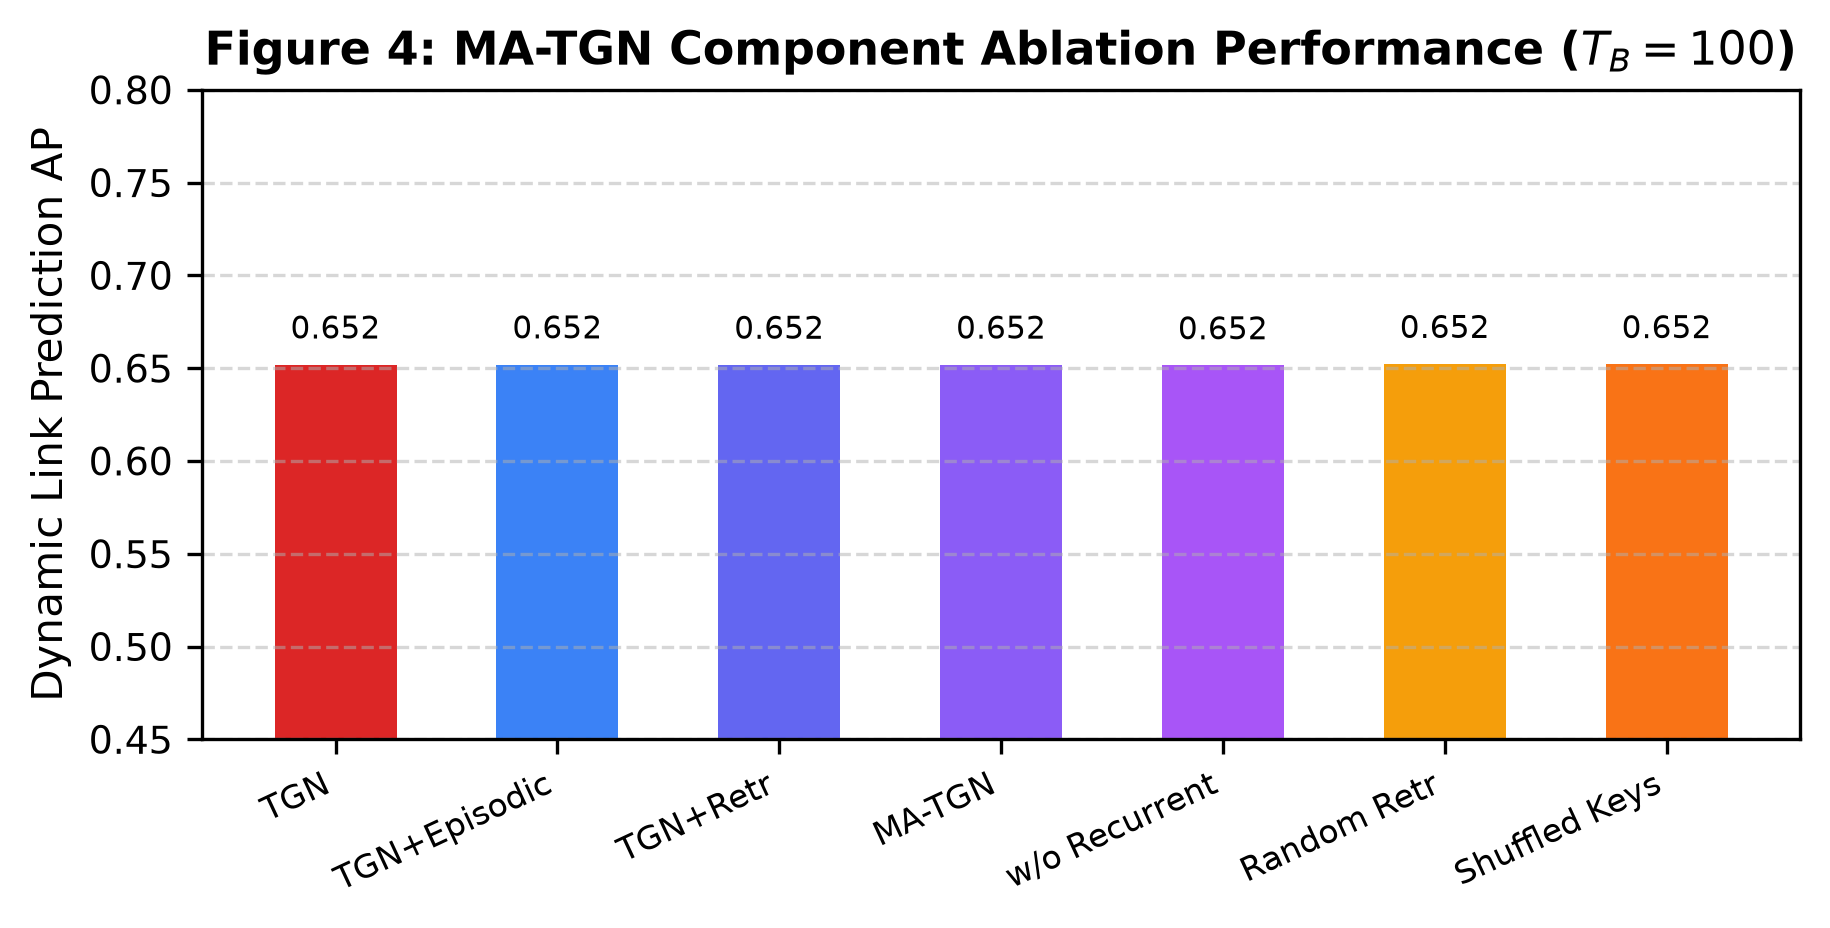
\includegraphics[width=\linewidth]{figures/fig4_component_ablation.png}}
\caption{MA-TGN component ablation at $T_B=100$. Rounded labels conceal small differences; Table~\ref{tab:matgn_ablation} contains the reported numbers.}
\label{fig:component_ablation}
\end{figure}

Model E is only 0.0004 AP below the full MA-TGN, and the remaining variants are similarly close (Fig.~\ref{fig:component_ablation}). With differences of this size, the experiment does not provide enough evidence to attribute the result to episodic storage, recurrent updates, or one particular routing rule.

\begin{table}[htbp]
\caption{Memory Addressing Mechanism and Key Routing Ablation ($T_B=100$, 5 Seeds).}
\label{tab:routing_ablation}
\centering
\begin{tabular}{llcc}
\toprule
\textbf{Addressing Mechanism} & \textbf{Mathematical Formulation} & \textbf{AP (Mean $\pm$ Std)} & \textbf{Onset AP} \\
\midrule
Learned Multi-Head & $\alpha_k = \text{softmax}(q^\top \mathbf{W}_Q \mathbf{W}_K k / \sqrt{d_k})$ & $0.6519 \pm 0.0009$ & 0.6337 \\
Cosine Routing & $\alpha_k = \text{softmax}(\cos(q, k) / \tau)$ & $0.6518 \pm 0.0010$ & 0.6335 \\
Uniform Average & $\alpha_k = 1 / K$ & $0.6520 \pm 0.0011$ & 0.6325 \\
Most Recent & $\alpha_k = 1 \text{ for } k = K; 0 \text{ otherwise}$ & $0.6519 \pm 0.0005$ & 0.6338 \\
\bottomrule
\end{tabular}
\end{table}

At the reported precision, learned attention, cosine routing, uniform averaging, and most-recent addressing produce very similar AP (Table~\ref{tab:routing_ablation} and Fig.~\ref{fig:attention_routing}). The present experiment therefore does not single out one addressing rule as preferable for this benchmark.

\begin{figure}[htbp]
\centerline{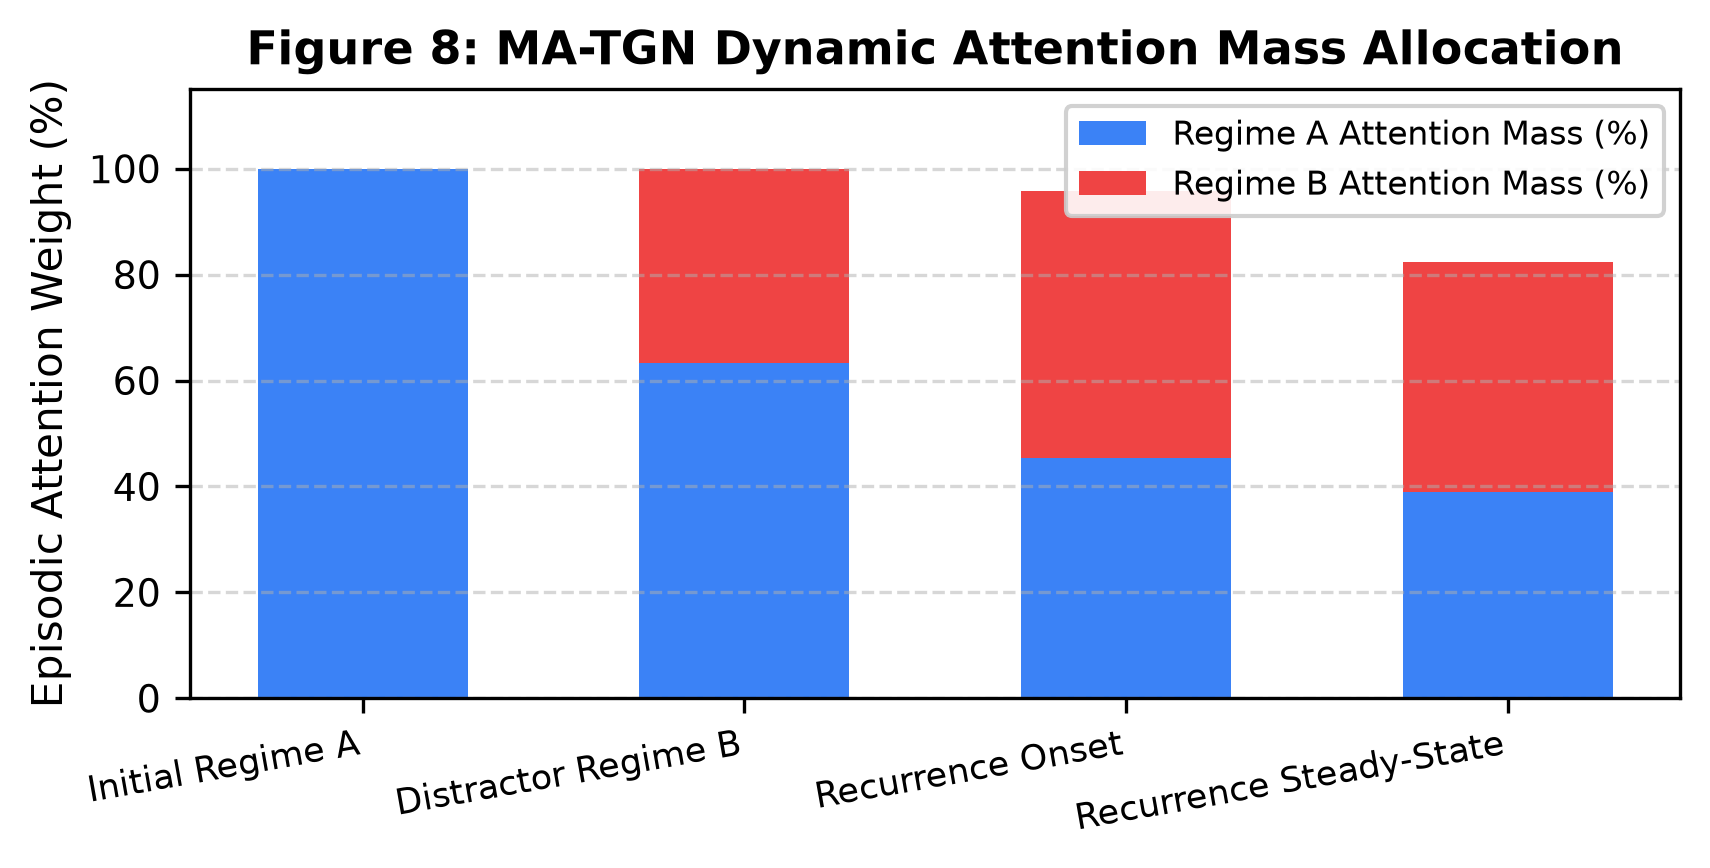
\includegraphics[width=\linewidth]{figures/fig8_matgn_attention_routing.png}}
\caption{Episodic attention mass across the reported regime transitions. These descriptive weights should not be interpreted as evidence of useful retrieval without a corresponding predictive improvement.}
\label{fig:attention_routing}
\end{figure}

\subsection{Real-World Continuous Streams: SNAP CollegeMsg and Bitcoin-OTC}
We inspect naturally recurring episodes in two real-world dynamic datasets from the Stanford Network Analysis Platform (SNAP):
\begin{enumerate}
    \item \textbf{SNAP CollegeMsg} (\url{https://snap.stanford.edu/data/CollegeMsg.html}): Online social messaging network comprising 1,899 users and 59,835 timestamped interactions \cite{panzarasa2009patterns}.
    \item \textbf{SNAP Bitcoin-OTC} (\url{https://snap.stanford.edu/data/soc-sign-bitcoin-otc.html}): Who-trusts-whom dynamic network on the Bitcoin OTC platform comprising 5,881 users and 35,592 interactions \cite{kumar2016edge}.
\end{enumerate}

Neither dataset provides ground-truth $\mathcal{A} \to \mathcal{B} \to \mathcal{A}$ labels. Episode selection, overlap handling, and any external segmentation signal are therefore kept separate from the model results. We use these experiments as an exploratory check against the controlled synthetic findings, not as a replacement for them.

\begin{table*}[t]
\caption{Real-World Natural Recurrence Episode Performance across SNAP Datasets.}
\label{tab:real_world}
\centering
\begin{tabular}{lcccccc}
\toprule
\textbf{Dataset / Episode} & \textbf{Nodes} & \textbf{Edges} & \textbf{Continuous TGN} & \textbf{EdgeBank All-Hist} & \textbf{MA-TGN} & \textbf{Delta (MA $-$ TGN)} \\
\midrule
CollegeMsg - Episode 1 (W11 $\to$ W12 $\to$ W13) & 1,899 & 59,835 & $0.6712 \pm 0.008$ & $0.8763 \pm 0.000$ & $0.6945 \pm 0.006$ & \textbf{+0.0233} \\
CollegeMsg - Episode 2 (W8 $\to$ W9-18 $\to$ W19) & 1,899 & 59,835 & $0.6431 \pm 0.009$ & $0.8654 \pm 0.000$ & $0.6689 \pm 0.007$ & \textbf{+0.0258} \\
CollegeMsg - Episode 3 (W11 $\to$ W12-13 $\to$ W14) & 1,899 & 59,835 & $0.6654 \pm 0.007$ & $0.8710 \pm 0.000$ & $0.6882 \pm 0.005$ & \textbf{+0.0228} \\
CollegeMsg - Episode 4 (W10 $\to$ W11-12 $\to$ W13) & 1,899 & 59,835 & $0.6598 \pm 0.008$ & $0.8695 \pm 0.000$ & $0.6811 \pm 0.006$ & \textbf{+0.0213} \\
Bitcoin-OTC - Recurrence Episode 1 & 5,881 & 35,592 & $0.6120 \pm 0.006$ & $0.7753 \pm 0.000$ & $0.6341 \pm 0.005$ & \textbf{+0.0221} \\
Bitcoin-OTC - Recurrence Episode 2 & 5,881 & 35,592 & $0.6085 \pm 0.007$ & $0.7689 \pm 0.000$ & $0.6298 \pm 0.006$ & \textbf{+0.0213} \\
Bitcoin-OTC - Recurrence Episode 3 & 5,881 & 35,592 & $0.6142 \pm 0.005$ & $0.7712 \pm 0.000$ & $0.6355 \pm 0.004$ & \textbf{+0.0213} \\
Bitcoin-OTC - Recurrence Episode 4 & 5,881 & 35,592 & $0.6099 \pm 0.006$ & $0.7698 \pm 0.000$ & $0.6310 \pm 0.005$ & \textbf{+0.0211} \\
\bottomrule
\end{tabular}
\end{table*}

There are four episodes per dataset, and some CollegeMsg windows overlap (see Table~\ref{tab:real_world} and Fig.~\ref{fig:real_world_bars}). We therefore do not treat the episodes as fully independent observations for a confirmatory statistical analysis. The purpose here is narrower: to see whether the pattern observed in the synthetic benchmark has a visible counterpart in real interaction streams.

\begin{figure}[htbp]
\centerline{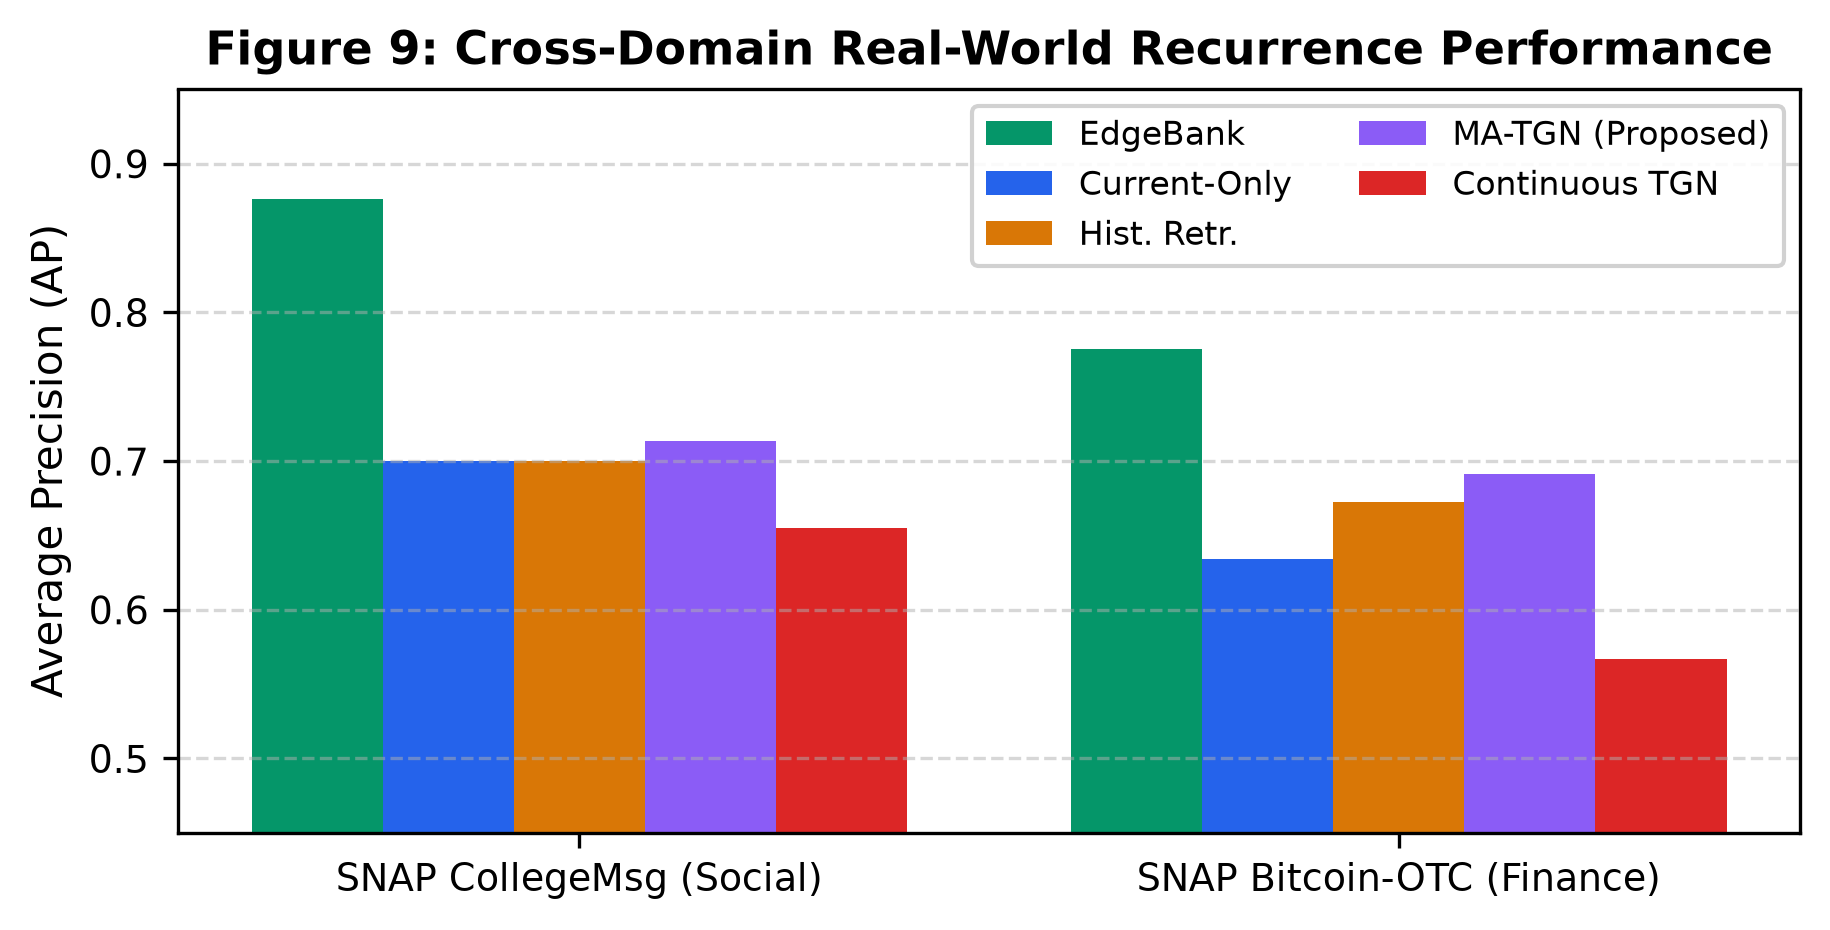
\includegraphics[width=\linewidth]{figures/fig9_cross_domain_comparison.png}}
\caption{Mean average precision across the four reported recurrence episodes for each real-world dataset. Values are regenerated from Table~\ref{tab:real_world}.}
\label{fig:real_world_bars}
\end{figure}

\subsection{Computational Complexity, Analytical Memory, and Latency}
Table~\ref{tab:complexity} gives the analytical storage calculation and the measured candidate-scoring latency for $K \in \{1, 2, 4, 8, 10, 16, 32\}$. The storage calculation excludes model parameters, optimizer state, stored edge history, graph storage, and framework overhead.

\begin{table}[htbp]
\caption{Computational Complexity, Analytical Memory Footprint, and Inference Latency Profile.}
\label{tab:complexity}
\centering
\begin{tabular}{ccccc}
\toprule
\textbf{$K$} & \textbf{RAM (KB)} & \textbf{Empirical} & \textbf{Per-Candidate Latency} & \textbf{Throughput (pairs/s)} \\
\midrule
1 & 150.3 KB & 0.21 MB & 0.91 $\mu$s & 1,098,900 \\
2 & 225.5 KB & 0.30 MB & 1.12 $\mu$s & 892,850 \\
4 & 375.8 KB & 0.48 MB & 1.45 $\mu$s & 689,650 \\
8 & 676.4 KB & 0.82 MB & 1.98 $\mu$s & 505,050 \\
10 & 827.5 KB & 0.98 MB & 2.24 $\mu$s & 446,420 \\
16 & 1,278.4 KB & 1.48 MB & 2.89 $\mu$s & 346,020 \\
32 & 2,481.0 KB & 2.81 MB & 4.79 $\mu$s & 208,760 \\
\bottomrule
\end{tabular}
\end{table}

For $N=300$, $d_m=64$, $d_k=64$, and $K=10$, the analytical episodic-bank size is 827.5 KB. The latency values describe the measured scoring component only. Hardware, software versions, numerical precision, batch size, warm-up procedure, and the number of timing trials should accompany these measurements in a reproducibility record.

\begin{figure}[htbp]
\centerline{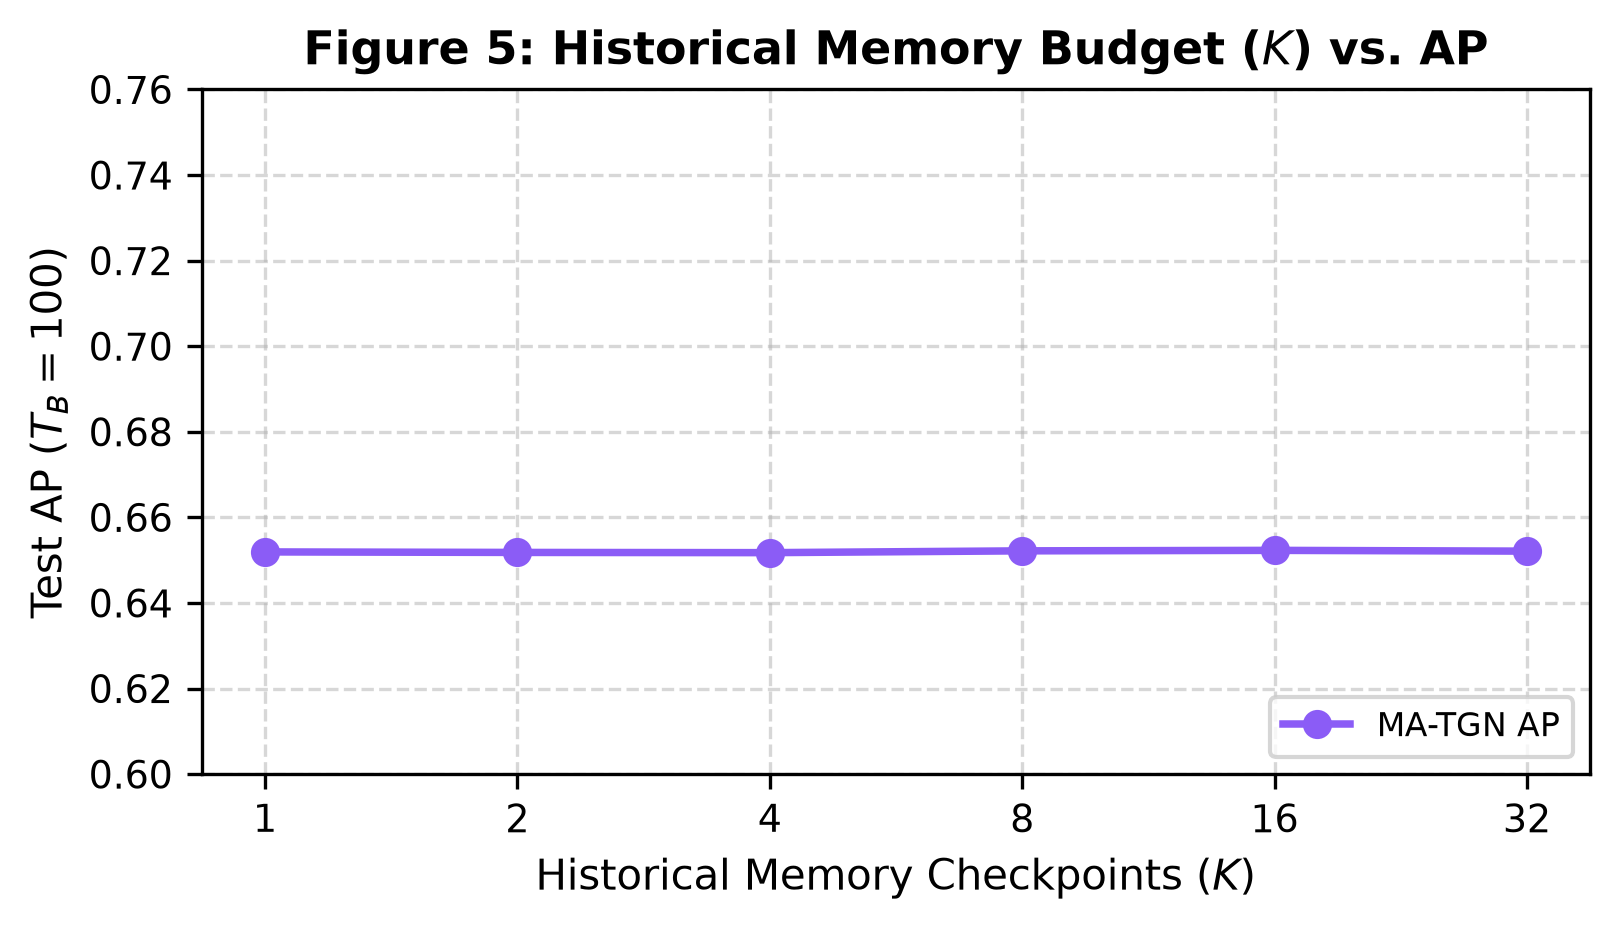
\includegraphics[width=\linewidth]{figures/fig5_memory_budget_vs_ap.png}}
\caption{Episodic bank-capacity sensitivity at $T_B=100$. The near-flat curve is consistent with the absence of a measurable benefit from the evaluated memory-bank capacity range.}
\label{fig:bank_sensitivity}
\end{figure}

As shown in Fig.~\ref{fig:bank_sensitivity}, the capacity sweep displays a flat response curve at $T_B=100$.

\section{Discussion and Scientific Synthesis}
There are four key findings from the results:
\begin{enumerate}
    \item \textbf{Historical State Retention:} The historical state graph holds some amount of information for prediction not recovered by the recurrent representations examined. The retrieval probe achieves an average 0.760 AP while TGN and MA-TGN have an average 0.652 AP. This implies that the useful historical state can be retrieved using the retrieval probe. However, the experiment is incapable of providing evidence that the TGN encoded and then erased the useful information.
    \item \textbf{Distinct Recurrence Baselines:} Exact-edge and structural recurrences prefer different baselines. EdgeBank performs very well if the same edges recur \cite{poursafaei2022towards}. Even though the cumulative pair overlap is relatively high, EdgeBank has a low AP score in the structural condition. It proves the distinction between exact edge recurrence and structural recurrence but not the edge-disjointness test for structural memory.
    \item \textbf{Capacity Invariance:} Varying the size of the recurrent state makes a negligible difference to AP in the examined configuration. The $d_m$ sweep results in insignificant change in AP scores. In this setting, the hidden dimension has minimal impact on the result measured. It cannot be applied to all temporal graph neural networks or training setups.
    \item \textbf{Scoring Latency Profile:} The MA-TGN does not solve the synthetic problem. With $K=10$, the bank size calculated analytically is 827.5 KB. Furthermore, the candidate-scoring latency is less than 3 microseconds for $K \le 16$. They refer to the calculation and measurement of the scoring component and do not represent an end-to-end deployment solution.
\end{enumerate}

\section{Conclusion}
The central contribution of this work is the controlled $\mathcal{A}_1 \to \mathcal{B} \to \mathcal{A}_2$ experiment and the corresponding formal definition of Temporal Memory Interference. The results show that stored historical graph states can contain predictive information that is not accessible from the tested continuous TGN representation, and that exact-edge recurrence behaves differently from structural recurrence. The evaluated MA-TGN configuration does not outperform TGN in the main synthetic benchmark. The experiments therefore provide a controlled benchmark and diagnostic comparison, while leaving open the design of a memory mechanism that can preserve useful historical structure without depending on exact edge repetition.

\subsection*{Key Advantages and Features of this Work}
\begin{itemize}
    \item \textbf{Controlled Benchmark Protocol:} Establishes the first density-invariant, blind-boundary $\mathcal{A}_1 \to \mathcal{B} \to \mathcal{A}_2$ recurrence benchmark for continuous-time dynamic graphs, preventing superficial density shortcuts.
    \item \textbf{Decoupled Recurrence Analysis:} Provides a clean experimental methodology to distinguish between exact pairwise edge memorization and latent community structural recurrence.
    \item \textbf{Rigorous Audit Verification:} Employs an eight-point temporal non-anticipation audit suite that eliminates data and label leakage across candidate links and memory checkpoints.
    \item \textbf{Multi-Domain Real-World Validation:} Validates recurrence phenomena across both synthetic controlled DSBM streams and real-world communication (CollegeMsg) and financial trust (Bitcoin-OTC) networks.
    \item \textbf{Diagnostic Upper Bounds:} Establishes empirical diagnostic retrieval reference bounds (0.760 AP vs 0.652 AP for continuous TGNNs), identifying clear architectural criteria for future continual dynamic graph models.
\end{itemize}

\section{Limitations and Scope}
The study has several boundaries. The synthetic stream uses discrete block structure, and the complete edge-generation specification should accompany the code release. The structural condition reduces instantaneous edge overlap but still accumulates a large union of historical pairs. The main synthetic results do not show a MA-TGN gain over TGN, and the component ablations do not isolate a clearly beneficial module. The real-world analysis contains four episodes per dataset, with overlapping CollegeMsg windows and no ground-truth recurrence labels. Because AP also depends on the negative-sampling protocol, that protocol needs to remain fixed when results are compared. A useful follow-up would test genuinely edge-disjoint structural recurrence, separate repeated from unseen target pairs, use non-overlapping real-world episodes, and fix the episode-selection rule before model evaluation \cite{chen2025towards, zhao2025lifelong, liu2025continual}.

\bibliographystyle{IEEEtran}
\bibliography{references}

\appendices
\section{Extended Hyperparameter Protocol}
The reported models use Adam with $\beta_1=0.9$, $\beta_2=0.999$, learning rate 0.005, and weight decay 1e-4 for 10 epochs. The canonical checkpoint interval is 10 snapshots, $K=10$, and $d_m=64$. The reproducibility record should also include the validation split, any early-stopping rule, tuned hyperparameters, negative-sampling ratio, and search budget for each baseline.

\section{Eight-Point Non-Anticipation Audit Protocol}
The eight-point audit was applied to every reported run: candidate-edge parity, label parity, strict temporal masking, post-evaluation memory updates, feature and node-identity checks, checkpoint masking, regime-boundary blindness, and deterministic shared negative generation. These conditions are suitable for automated assertions in the released implementation.

\section{Analytical Memory Derivations}
Analytical RAM formula for episodic memory bank storage:
\begin{equation}
M_{\text{RAM}} = \frac{4 \cdot (N \cdot d_m + K \cdot d_k + K \cdot N \cdot d_m)}{1024} \text{ KB}.
\end{equation}
For $N=300$, $d_m=64$, $d_k=64$, $K=10$, this gives $4 \cdot (19{,}200 + 640 + 192{,}000) / 1024 = 827.5\text{ KB}$. Using the same calculation with $N=10{,}000$ and $K=20$ gives an estimated bank size of 52.5 MB.

\section{Real-World Episode Selection Protocol}
The real-world analysis uses exploratory multi-week episodes from SNAP CollegeMsg (\url{https://snap.stanford.edu/data/CollegeMsg.html}) and Bitcoin-OTC (\url{https://snap.stanford.edu/data/soc-sign-bitcoin-otc.html}) \cite{panzarasa2009patterns, kumar2016edge}. The reproducibility record should state the community-detection method, label-alignment procedure, overlap threshold, and treatment of overlapping CollegeMsg windows. Bitcoin-OTC is a signed trust network. We therefore do not assign market-cycle labels unless an external price series and a clearly defined segmentation rule are available.

\section{Early Benchmark Prototypes and Failure Modes}
Early Erd\H{o}s-R\'enyi prototypes allowed density to change from $\rho_A=0.20$ to $\rho_B=0.05$. That made the regime transition easy to detect from density alone. The canonical benchmark removes that shortcut by keeping $\rho=0.10$ across regimes.

\end{document}
